%% ---------------------------------------------------------------------------------------------------------------------

\chapter{\textit{go-geiger}: Identification of \textit{Unsafe} Usage}\label{ch:go-geiger}

This chapter presents \toolGeiger{}, a tool to find usages of the \unsafe{} \acrshort{API} in Go packages and their
dependencies.
Figure~\ref{fig:outline4} shows an outline of the contents of this chapter.
Using open-source projects from \github{} and \toolGeiger{}, an empirical study on \unsafe{} usage is done, which is
used additionally to quantitatively evaluate \toolGeiger{}.
Furthermore, a novel data set of labeled samples of \unsafe{} code is described and used as a qualitative analysis on
\unsafe{} usage in Go.

\begin{figure}[ht]
    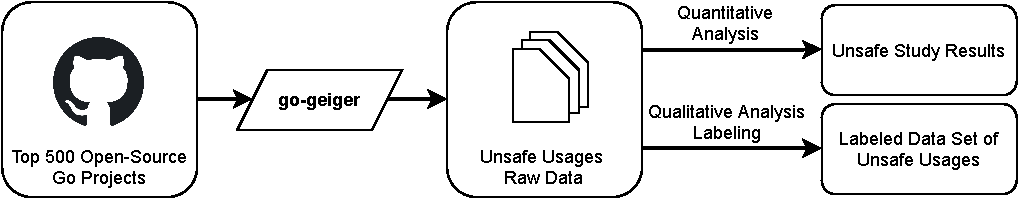
\includegraphics[width=\textwidth]{assets/figures/chapter4/outline4.pdf}
    \caption{Role of Chapter 4 in Thesis Outline}
    \label{fig:outline4}
\end{figure}



%% ---------------------------------------------------------------------------------------------------------------------

\section{Design}\label{sec:go-geiger:design}

The novel tool \toolGeiger{} is designed to identify usages of the \unsafe{} \acrshort{API} in Go source code.
It is available on \github{}\footnote{\url{https://github.com/jlauinger/go-geiger}}.
The tool includes the dependencies of Go packages in its analysis, which gives a more complete picture of possible
\unsafe{} usages than only looking at an individual package.
It is inspired by \toolCargoGeiger{}\footnote{\url{https://github.com/rust-secure-code/cargo-geiger}}, a similar tool
for detecting the use of \unsafe{} code blocks in Rust programs.

\begin{figure}[htp!]
    %\vspace{2mm}
    \centering
    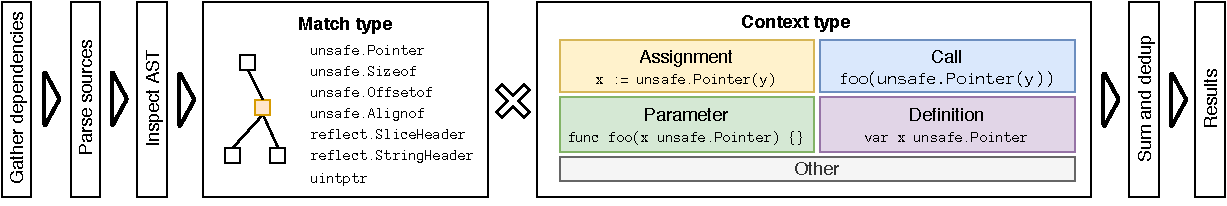
\includegraphics[width=\textwidth]{assets/figures/chapter4/go-geiger-architecture.pdf}
    \caption{Architecture of the \toolGeiger{} tool to detect unsafe usages}
    \label{fig:geiger-architecture}
    %\vspace{-10pt}
\end{figure}


Figure~\ref{fig:go-geiger-architecture} shows the architecture of \toolGeiger{}.
First, it determines the scope of code that should be analyzed for \unsafe{} usage.
To achieve this, the dependency tree of the packages given to \toolGeiger{} is built.
Then, the sources of all the packages in this tree are parsed, and the resulting abstract syntax trees (\acrshort{AST})
are inspected.
Within the \acrshort{AST}, usages of the \unsafe{} \acrshort{API} are identified.
Each usage is assigned a tuple of labels consisting of \textit{match type} and \textit{context type}.
The match type represents the part of the \unsafe{} \acrshort{API} that is used.
It can be one of the four \unsafe{} package members \textit{Pointer}, \textit{Alignof}, \textit{Offsetof}, and
\textit{Sizeof}, the \textit{reflect} package fields \textit{SliceHeader} and \textit{StringHeader}, or the
\textit{uintptr} keyword.
The context type indicates the functional part of code that the usage is found in.
It can be either an \textit{assignment}, a \textit{call} to a function, a function \textit{parameter} definition, or a
\textit{variable} definition.
Context identification is done based on the abstract syntax tree (\acrshort{AST}), which might lead to edge cases in
some programs that are not handled by \toolGeiger{}.
For example, this could happen if future releases of Go introduce new \acrshort{AST} node types.
To mitigate this possibility, the context is set to \textit{other} in \toolGeiger{} if all four other options can not be
applied.
The context allows to filter the search for \unsafe{} usages in particular functional code positions.
For example, it is possible to find only \unsafe{} usages that are used within parameters of function calls.
After the \unsafe{} usages are identified, they are counted.
For this, it is necessary to take care of package deduplication.
If a particular package exists in the dependency tree multiple times and is reachable on different paths, it must still
be counted only once when calculating the sum of \unsafe{} usages in a package's dependencies.
This is because the package does not get any less safe by including the same code multiple times.
The code is already part of the resulting program.
Finally, the analysis results are shown to the user.

\begin{figure}[htp!]
    %\vspace{2mm}
    \centering
    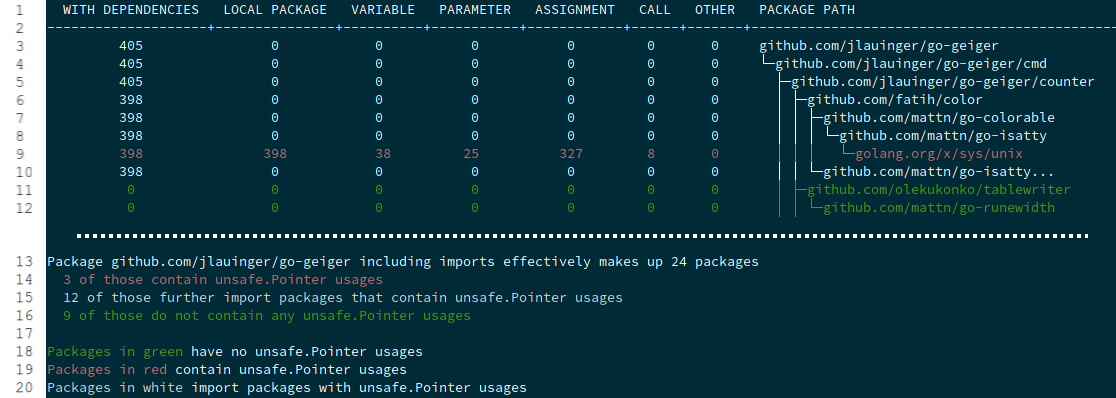
\includegraphics[width=\textwidth]{assets/images/chapter4/go-geiger-screenshot.png}
    \caption{Usage example screenshot of \toolGeiger{}}
    \label{fig:go-geiger-screenshot}
    %\vspace{-14pt}
\end{figure}


Figure~\ref{fig:go-geiger-screenshot} shows a screenshot of \toolGeiger{}.
It presents the analyis results for the \textit{go-geiger} source code itself.
However, to decrease the space needed to display the figure, parts of the table with \unsafe{} counts have been
excluded.
The output is composed of three sections.
The first is a table showing the \unsafe{} usage counts for each package in the dependency tree for the packages
given for analysis (Lines~1--12).
The first column indicates the total number of usages in the package including all its dependencies.
The second column shows the number for the package itself, without the dependencies.
The heading for this column is \textit{local package}.
Next, there are five columns with individual usage counts for the possible context types described above.
These columns add up to the \textit{local package} count.
Finally, the import path for the package is given to identify it.
Lines that are printed in green (Lines~11 and~12 in Figure~\ref{fig:go-geiger-screenshot}) represent packages with no
local \unsafe{} usages.
Red lines (Line~9) are packages that directly contain \unsafe{} code, and white lines (e.g.~Line~3) indicate that the
package does not contain \unsafe{} usages itself, but introduces them through its dependencies.
After the table, a summary of the number of packages belonging into these three categories is shown (Lines~13--16).
The output concludes with a legend for the colors (Lines~18--20).


%% ---------------------------------------------------------------------------------------------------------------------

\section{Implementation}\label{sec:go-geiger:implementation}

The identification of the dependency trees for the packages to analyze, as well as the parsing of the source code, is
done using the standard Go compiler toolchain.
It is accessable using the \textit{packages}
\acrshort{API}\footnote{\url{https://pkg.go.dev/golang.org/x/tools/go/packages}}.
Similarly, the inspection of the \acrshort{AST} is done using the \acrshort{API} available through the \textit{ast}
package in Go\footnote{\url{https://golang.org/pkg/go/ast/}}.

To find \unsafe{} usages corresponding to the different match types shown in Figure~\ref{fig:go-geiger-architecture},
the \acrshort{AST} is filtered for selector expressions (\textit{SelectorExpr} nodes) and identifiers (\textit{Ident}
nodes).
The first indicate possible usages of \textit{unsafe.Pointer}, \textit{Alignof}, \textit{Offsetof}, \textit{Sizeof},
\textit{reflect.SliceHeader}, or \textit{StringHeader}.
The second is used to find instances of \textit{uintptr}.
In both cases, the concrete identifier names in the \acrshort{AST} nodes are checked to distinguish \unsafe{} usages from
arbitrary other field accesses.
The context type is determined by going up in the \acrshort{AST} starting at the expression node corresponding to a
given \unsafe{} usage.
For example, an \unsafe{} usage is considered part of the \textit{assignment} context type if it is a descendent of
either an assignment statement (\textit{AssignStmt} node), composite literal (\textit{CompositeLit}), or return
statement (\textit{ReturnStmt}).
The \textit{call}, \textit{parameter}, and \textit{variable} classes correspond to call expression (\textit{CallExpr}),
function declaration (\textit{FuncDecl}), and general declaration (\textit{GenDecl}) nodes, respectively.
To achieve an effective assignment of the context type, the order in which the different types are checked is important.
This is because an \unsafe{} usage could be included in several context types in an example like
\textit{x~:=~f(unsafe.Pointer(y))}.
The \acrshort{AST} for this statement consists of an assignment statement, where the right hand side is a call
expression.
This call expression contains the \unsafe{} usage.
Therefore, by ascending in the \acrshort{AST} and depending on the order of checking, both context types \textit{call}
and \textit{assignment} could be applied.
Which order should be used is a design decision, and for \toolGeiger{} it is \textit{assignment}, \textit{call},
\textit{parameter}, and finally \textit{variable}.

The \unsafe{} usage counts are first collected individually for every package.
A cache is used to avoid analyzing the same package multiple times if it is present multiple times in the dependency
tree.
This cache is aware of possibly different versions of the same package and stores them separately.
When the usage count including dependencies is calculated, \toolGeiger{} starts with the root packages that were
requested for analysis by the user, and recursively calculates the respective counts.
Again, the cache is used to avoid summing up multiple times.
This approach is a depth-first traversal of the dependency tree.


%% ---------------------------------------------------------------------------------------------------------------------

\section{Quantitative Evaluation}\label{sec:go-geiger:quantitative-evaluation}

To evaluate \toolGeiger{} on real-world code, it is used to gather empirical data about the usage of \unsafe{} in
popular open-source Go projects.
This section presents a study which was designed to answer the following research questions:

\begin{enumerate}[left=0.5cm, label={RQ\arabic*}]
    \item How prevalent is \unsafe{} in Go projects? \label{rq:prevalApp}
    \item How deep are code packages using \unsafe{} buried in the dependency tree? \label{rq:depsDepth}
    \item Which \unsafe{} keywords are used most? \label{rq:distTypes}
    \item Does \unsafe{} usage correlate to project metrics such as age or popularity? \label{rq:popularity}
    \item How does the use of \unsafe{} change over the lifetime of the code? \label{rq:changeTime}
    \item Does \toolGeiger{} provide additional insights into \unsafe{} usage compared to other linters? \label{rq:linterComparison}
    \item Which \unsafe{} operations are used in practice, and for what purpose? \label{rq:purpose}
\end{enumerate}

The following subsections first discuss how the data for this study was gathered, and then answer research
questions~\ref{rq:prevalApp} to~\ref{rq:linterComparison}.
Section~\ref{subsec:go-geiger:qualitative-evaluation:purpose} presents the answer to~\ref{rq:purpose}.
It is answered later, because it is based on a novel, manually labeled data set of \unsafe{} usage purposes, which is
introduced in Section~\ref{subsec:go-geiger:qualitative-evaluation:labeled-dataset}.


%% ---------------------------------------------------------------------------------------------------------------------

\subsection{Data Set}\label{subsec:go-geiger:evaluation:data-set}

To build a data set of \unsafe{} usages, first the top \projsTotal{} most-starred open-source Go projects available on
\github{} were downloaded.
This initial download was done on \checkNum{May 27, 2020}.
These \projsTotal{} projects with their respective revisions are listed in the appendix (Table~\ref{tbl:projects}).
Since \toolGeiger{} is specifically built to analyze the project dependencies, all projects that do not support the Go
modules system were removed from the set.
This is necessary to ensure that all dependencies can be automatically resolved and the respective sources are available
for analysis.
There were \projsWithoutModules{} projects that had no support for modules.
They are indicated in Table~\ref{tbl:projects} by the \textit{nm} label in the last column.
Furthermore, \projsNotCompiled{} projects could not be compiled and thus also had to be excluded from the data set.
The \textit{bf} label is used in the appendix table to mark those projects.
Since \toolGeiger{} analyzes the \acrshort{AST}, it can not work on packages that can not be parsed.
This results in a set of \projsAnalyzed{} Go projects.
These have between \checkNum{3,075} and \checkNum{72,988} stars, with an average of \checkNum{7,860}.

As a next step, the dependency trees for all projects selected for analysis were built, resulting in \packagesAnalyzed{}
unique packages.
These consist of \checkNum{186} packages that are part of the Go standard library, and \checkNum{61,839} which are not.
The average size of the packages is \checkNum{1,402} lines of code (\acrshort{LOC}), with a standard deviation of
\checkNum{5,612}, in \checkNum{4.4} Go files on average (standard deviation \checkNum{11.3}).
These packages were analyzed using \toolGeiger{}, as well as the existing static analysis tools \toolVet{} and
\toolGosec{} to allow a comparison between the findings of these tools.
The resulting findings were stored in machine-readable \acrshort{CSV} files.
The data set contains \uniqueUnsafeFindings{} unique \unsafe{} usages.
All data files as well as the data acquisition tool used to download the projects and run the analysis tools are
available in a data repository on \github{}\footnote{\url{https://github.com/stg-tud/unsafe_go_study_results}}.
Additionally, the data repository\footnote{\url{https://zenodo.org/record/4107497}} and the raw projects source
code\footnote{\url{https://zenodo.org/record/4001728} \todo{update and check}} are published on \zenodo{}.


%% ---------------------------------------------------------------------------------------------------------------------

\subsection{\textit{Unsafe} Usages in Projects and Dependencies (\ref{rq:prevalApp},~\ref{rq:depsDepth},~\ref{rq:distTypes})}\label{subsec:go-geiger:evaluation:unsafe-usage}

To attribute \unsafe{} usages to either a project or one of its dependencies, the root module of the project is used.
Since the data set was constructed such that all projects support the Go module system as described in the previous
section, there is a top-level \textit{go.mod} file present for each of them.
The module specified in that file is stored as the project root.
Packages that are part of this module are (first-party) project code.
Other packages that are present in the dependency tree, but not in the root module, are (third-party) dependencies.

By looking at \unsafe{} findings that are part of first-party packages, it is possible to determine how many projects
directly use \unsafe{} in their code.
The data shows that this is the case for \unsafeProjects{} (\percentageUnsafeProjects{}) of the \projsAnalyzed{}
projects.
However, this does not take the dependencies into account.
With respect to these, \unsafeTransitiveWithDependencies{} (\percentageUnsafeTransitiveWithDependencies{}) of the
projects transitively import \unsafe{} usages.
To calculate this percentage, the complete dependency trees of the projects are integrated into the analysis.
This results in \packagesAnalyzed{} unique packages, \unsafePackages{} (\percentageUnsafePackages{}) of which contain at
least one \unsafe{} usage.
This answers research question~\ref{rq:prevalApp} about the prevalence of \unsafe{} in Go projects.

The fraction of projects importing \unsafe{} in the previous paragraph does not include the Go standard library.
All analyzed projects import this library and it contains \unsafe{} usages, which means that with it \checkNum{100\%} of
the projects would transitively use \unsafe{}.
Because the standard library is developed by the Go core team, it can be assumed that it is well audited and reasonably
safe to use.
Since there is no way to exclude it from a project anyways, the analysis presented in this study is more meaningful
when the standard library is not causing a project to be counted as using \unsafe{}.

\begin{answerToRQ}[\ref{rq:prevalApp}]
    About \percentageUnsafeProjectsRounded{} of projects contain \unsafe{} usages in their first-party code.
    Approximately \percentageUnsafeTransitiveWithDependenciesRounded{} of projects transitively import at least one
    third-party dependency package with \unsafe{} usages.
\end{answerToRQ}

To answer research question~\ref{rq:depsDepth} about how deep in the dependency tree packages using \unsafe{} are
usually located, the import depth of all packages used by a project is determined.
Import depth denotes the minimum depth of a package in the dependency tree of a particular project, which is the
shortest path from the project root module to the package.
Thus, all packages included in the root module have an import depth of \checkNum{zero}.
Packages which are imported by those have a depth of \checkNum{one}, and so on.
The depth is calculated using breadth-first search on the dependency tree, which saves time when packages are imported
multiple times because the analysis is focused on the mimimum.
Figure~\ref{fig:unsafe-import-depth} presents a heatmap plot of the number of packages containing \unsafe{} usages by
their import depth.
The y-axis denotes the depth, the color intensity shows the number of packages using \unsafe{} at a given depth, and the
x-axis represents the \projsAnalyzed{} analyzed projects.
On the left hand side, next to the heat map, the horizontal bar chart visualizes the total number of packages at each
import depth summed up over all projects.
Packages that do not contain any \unsafe{} usages are not included in the sum as they are irrelevant for
answering~\ref{rq:depsDepth}.

\begin{figure*}[!t]
    \vspace{2mm}
    \centering
    %\includegraphics[width=\textwidth]{gfx/figures/unsafe-import-depth.pdf}
    \includegraphics[width=.9\textwidth]{gfx/figures/unsafe-import-depth.pdf}
    \caption{Import Depth of Unsafe Packages. Unsafe packages are around a depth of \averageUnsafeImportDepth{} (sd=\stdUnsafeImportDepth{})}
    \label{fig:unsafe-import-depth}
    %\vspace{-10pt}
\end{figure*}


Figure~\ref{fig:unsafe-import-depth} shows that most packages containing \unsafe{} usages are imported fairly early,
however not directly at the first level.
The average depth is \averageUnsafeImportDepth{} with a standard deviation of \stdUnsafeImportDepth{}.
The general import depth of all packages, whether they contain \unsafe{} or not, is only slightly lower at
\averageGeneralImportDepth{}.
While the numbers are fairly low, the count of packages at each level of import depth increases exponentially.
Thus, while being possible, it is hard for developers to manually audit dependency packages for \unsafe{} usages.
The novel \toolGeiger{} tool helps by quickly identifying the packages containing \unsafe{}, therefore, it is possible
to conduct a focused review of the \unsafe{} code.
Only the first level of dependencies contains the packages that the project developers added themselves, thus, they are
obvious to them.
In the data set, \levelOneImportedUnsafePackagesCount{} (\levelOneImportedUnsafePackagesShare{}) of the
\unsafePackages{} packages containing \unsafe{} are imported at level one of the dependency tree, and
\levelZeroImportedUnsafePackagesCount{} (\levelZeroImportedUnsafePackagesShare{}) are not imported (level zero).
This further shows that the majority of \unsafe{} code is introduced further down in the dependency tree.

\begin{answerToRQ}[\ref{rq:depsDepth}]
    Most imported packages with at least one \unsafe{} usage are located around a depth of
    \averageUnsafeImportDepthRounded{} in the dependency tree.
\end{answerToRQ}

Research question~\ref{rq:distTypes} is about which \unsafe{} tokens are used the most.
As described in Section~\ref{sec:go-geiger:design}, \toolGeiger{} identifies usages of the four members of the \unsafe{}
package, the \textit{reflect.SliceHeader} and \textit{reflect.StringHeader} types, and \textit{uintptr}.
Figure~\ref{fig:unsafe-tokens-distribution} shows the distribution of these \unsafe{} types in the data set of Go
projects.

\begin{figure}[!t]
    \centering
    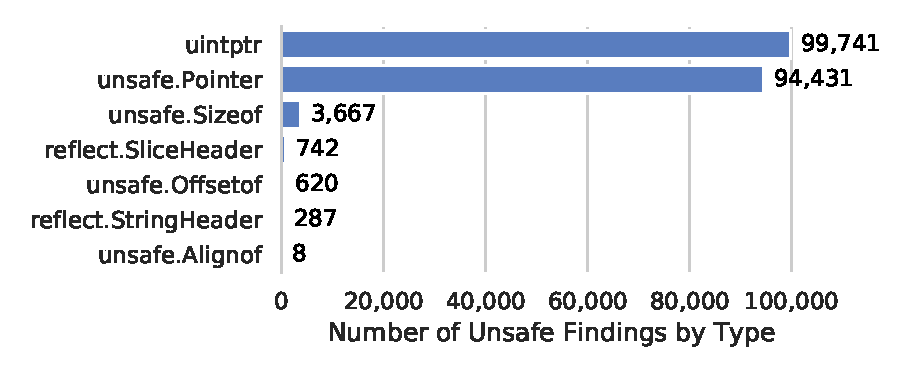
\includegraphics[width=0.43\textwidth]{assets/plots/distribution-unsafe-types.pdf}
    \caption{Distribution of different types of unsafe tokens}
    \label{fig:unsafe-tokens-distribution}
\end{figure}

The data shows that \textit{uintptr} is the most common \unsafe{} token, with \checkNum{99,741} findings.
Next, \textit{unsafe.Pointer} has a similarly high prevalence of \checkNum{94,431} samples.
These two lead the usage counts by far, with the next being \textit{unsafe.Sizeof} at only \checkNum{3,667} usages and
all other token types found less than \checkNum{1,000} times.
With a mere \checkNum{8} usages found, \textit{unsafe.Alignof} is the most rare.

\begin{answerToRQ}[\ref{rq:distTypes}]
    In the wild, \textit{uintptr} and \textit{unsafe.Pointer} are orders of magnitude more common than other \unsafe{}
    usages.
\end{answerToRQ}


%% ---------------------------------------------------------------------------------------------------------------------

\subsection{Influence of Age and Popularity (\ref{rq:popularity})}\label{subsec:go-geiger:evaluation:popularity}

This subsection answers research question~\ref{rq:popularity} about whether there is a correlation between \unsafe{}
usage and the common projects metrics age and popularity.
Popularity is measured by the number of stars and number of forks that a project has on \github{}.
Figure~\ref{fig:correlation-popularity} presents a scatter plot showing the number of \unsafe{} usages on the x-axis and
the project metrics stars, forks, and age on the y-axis.
Usages that are part of the Go standard library are not counted in this graph.
Each data point represents one project.
Blue circles indicate a project's number of stars, orange diamonds show the number of forks, and green crosses denote
the age.

\begin{figure}[htp!]
    %\vspace{2mm}
    \centering
    \includegraphics[width=\textwidth]{assets/plots/chapter4/unsafe-import-depth.pdf}
    \caption{TODO: Correlation between \unsafe{} usage and project metrics age and popularity}
    \label{fig:correlation-popularity}
    %\vspace{-10pt}
\end{figure}


Overall, the plot shows a uniform distribution between \unsafe{} usages and the different project metrics, except for
a gap between a \checkNum{few hundred} and \checkNum{1,000} usages of \unsafe{}.
There are both many projects with fewer and with more usages, but none with about \checkNum{750}.
This could be an indicator that once projects have included at least a couple of \unsafe{} usages, they tend to have
a lot of them rather easily.
There is no obvious correlation between neither \unsafe{} usage and project age, nor number of stars or forks.

\begin{answerToRQ}[\ref{rq:popularity}]
    There is no significant correlation between the number of \unsafe{} usages and a project's age, number of stars, or
    number of forks.
\end{answerToRQ}


%% ---------------------------------------------------------------------------------------------------------------------

\subsection{Change of \textit{Unsafe} Usage over Time (\ref{rq:changeTime})}\label{subsec:go-geiger:evaluation:over-time}

The data set collected in this study contains one version of each analyzed project.
It is not directly possible to measure the change of \unsafe{} usage in projects over time with the data available.
However, there are a number of modules that are included in several versions by different projects, which means that
these modules allow such an analysis of changes in \unsafe{} usage.
To answer research question~\ref{rq:changeTime}, this subsection discusses the differences between different versions of
four selected modules.
These modules are \textit{golang.org/x/sys}, \textit{github.com/golang/protobuf}, \textit{github.com/docker/docker}, and
\textit{k8s.io/apimachinery}.

\begin{figure}[ht!]
    \centering

    \begin{subfigure}[t]{0.475\textwidth}
        \centering
        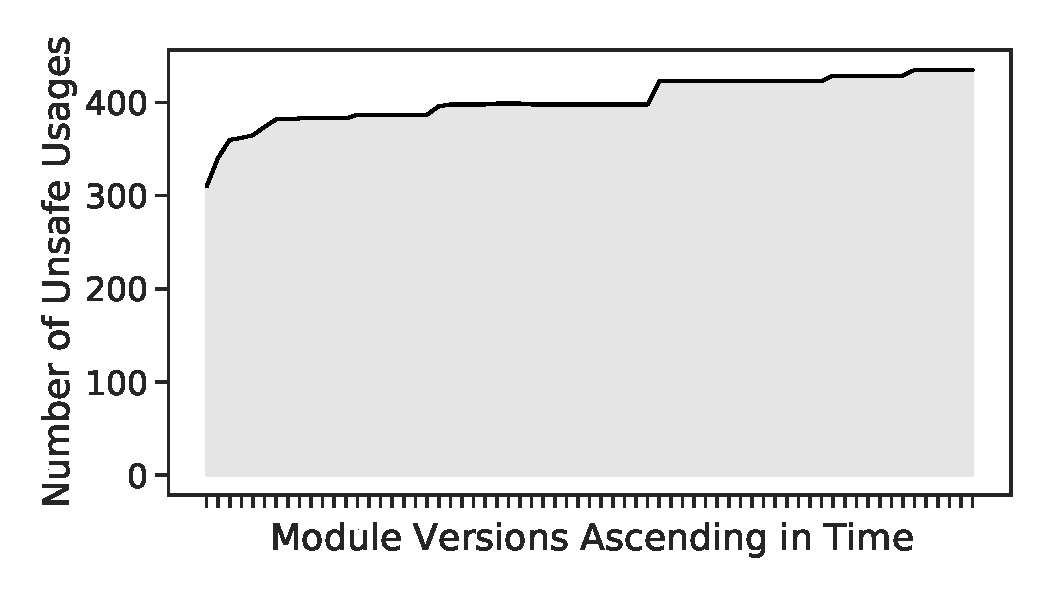
\includegraphics[width=\textwidth]{assets/plots/chapter4/unsafe-over-time-sys.pdf}
        \caption{\textit{golang.org/x/sys}}
        \label{subfig:change-over-time:sys}
    \end{subfigure}
    \hfill
    \begin{subfigure}[t]{0.475\textwidth}
        \centering
        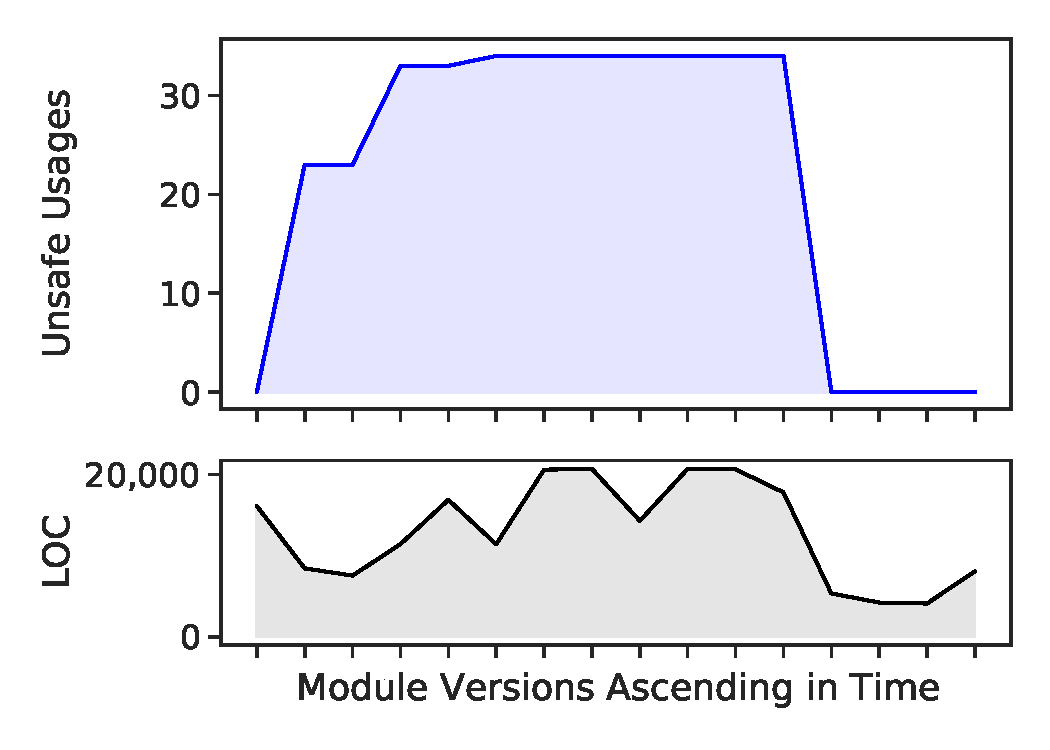
\includegraphics[width=\textwidth]{assets/plots/chapter4/unsafe-over-time-protobuf.pdf}
        \caption{\textit{github.com/golang/protobuf}}
        \label{subfig:change-over-time:protobuf}
    \end{subfigure}
    \vskip\baselineskip
    \begin{subfigure}[t]{0.475\textwidth}
        \centering
        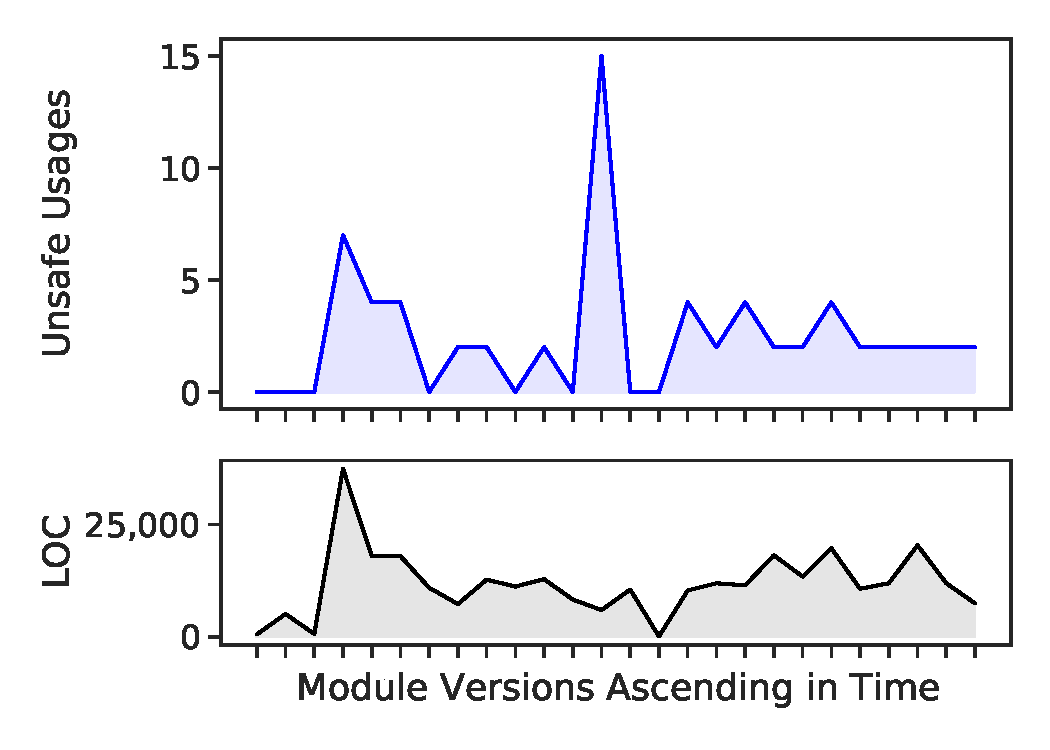
\includegraphics[width=\textwidth]{assets/plots/chapter4/unsafe-over-time-docker.pdf}
        \caption{\textit{github.com/docker/docker}}
        \label{subfig:change-over-time:docker}
    \end{subfigure}
    \hfill
    \begin{subfigure}[t]{0.475\textwidth}
        \centering
        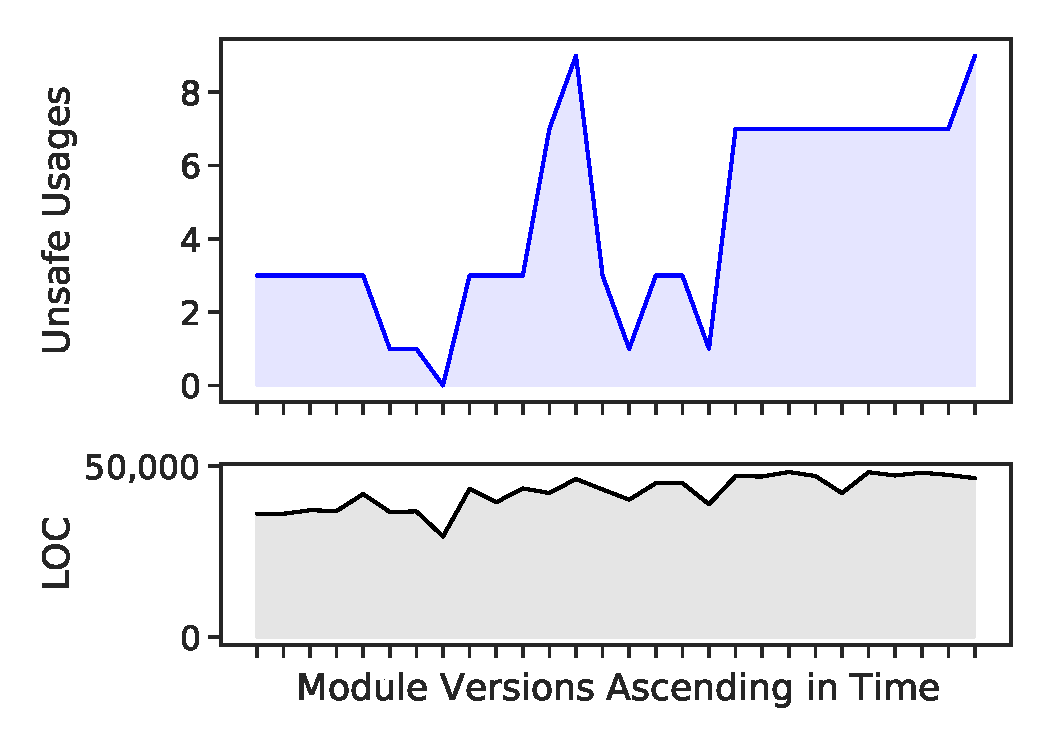
\includegraphics[width=\textwidth]{assets/plots/chapter4/unsafe-over-time-apimachinery.pdf}
        \caption{\textit{k8s.io/apimachinery}}
        \label{subfig:change-over-time:apimachinery}
    \end{subfigure}

    \caption[Change of \unsafe{} usage in selected packages over time]
        {Change of \unsafe{} usage in selected packages over time.\newline~Note different scaling on y axes.}
    \label{fig:change-over-time}
\end{figure}


Figure~\ref{fig:unsafe-over-time} shows the number of \unsafe{} usages contained in these modules by their respective
versions in blue, ascending over time.
Furthermore, the number of lines of code (\acrshort{LOC}) is plotted in gray to show possible correlations with changes
in module size.
It is important to note that the y axes in Figure~\ref{fig:unsafe-over-time} are scaled differently.
This is because the purpose of that figure is not to compare the modules against each other, but to see changes in their
usage of \unsafe{} over time.

Depending on the specific module, there are different conclusions.
For the \textit{golang.org/x/sys} module (Figure~\ref{subfig:unsafe-over-time:sys}), it is evident that there is a
monotonous increase both in \unsafe{} usage and \acrshort{LOC}.
The number of \unsafe{} usages increases from \sysModuleLeastUnsafe{} to \sysModuleMostUnsafe{}
(\sysModuleUnsafeIncrease) over the period shown in the figure, which is from \checkNum{late 2017} to
\checkNum{May 2020} (\checkNum{2.5 years}).
A manual analysis of the changes in the module source code shows that the increased usage of \unsafe{} in this case is
caused by additional system call \acrshort{API}s that are supported by the module.
Dispatching to the underlying system call code requires the use of \textit{unsafe.Pointer}.
Therefore, in this case more features provided by a dependency cause more \unsafe{} code to be imported into a project.

In the \textit{github.com/golang/protobuf} module (Figure~\ref{subfig:unsafe-over-time:protobuf}), there is initially a
steep increase in \unsafe{} usage, although the module size (\acrshort{LOC}) is decreasing.
Then, the number stays fairly constant until it drops to zero.
Thus, the module does not use \unsafe{} any longer, while the \acrshort{LOC} are increasing again.
It can be concluded that the module developers have replaced \unsafe{} with alternative, safe features of Go.

The \textit{github.com/docker/docker} module (Figure~\ref{subfig:unsafe-over-time:docker}) shows fluctuations in the use
of \unsafe{}, which are somewhat correlated to the module size (\acrshort{LOC}).
However, there is a big spike in \unsafe{} usage which is not reflected in the \acrshort{LOC} at all.
Also, the number of \unsafe{} usages overall is fairly low in this module.
The last module, \textit{k8s.io/apimachinery} (Figure~\ref{subfig:unsafe-over-time:apimachinery}), is similar.
Its \unsafe{} usage also has a limited correlation to the \acrshort{LOC}, but contains deviations.
Here, \unsafe{} has become more used in the module over time.
Still, it is only a very small fraction of the module size, which has almost \checkNum{50,000} \acrshort{LOC}.

In conclusion, the usage of \unsafe{} changes between different versions of the same module.
Therefore, it is important for developers to consider this when updating dependencies.
Furthermore, security analyses must be done for each version of a module.
It is not sufficient to determine that \unsafe{} usages do not enable vulnerabilities once, instead it must be checked
for the specific version that is imported into an application.

\begin{answerToRQ}[\ref{rq:changeTime}]
    Changes in \unsafe{} usage in particular modules are motivated, for example, by new \acrshort{API} requirements and
    can be significant, with about a \sysModuleUnsafeIncreaseRounded{} increase over \checkNum{2.5} years found in the
    \textit{sys} module.
    Since there is ongoing fluctuation in the usage of \unsafe{} over time for specific modules, security analyses must
    be done for each version individually.
\end{answerToRQ}


%% ---------------------------------------------------------------------------------------------------------------------

\subsection{Comparison with Existing Tools (\ref{rq:linterComparison})}\label{subsec:go-geiger:evaluation:linters-comparison}

To evaluate the benefit \toolGeiger{} provides in comparison to existing static analysis tools for Go, its findings are
put in context with the results of \toolVet{} and \toolGosec{} in this section.
The goal of this comparison is to see whether any of those tools can achieve the same as \toolGeiger{} does.
As described in Section~\ref{sec:background:static-code-analysis}, \toolVet{} is a linter that is included as part of
the standard Go command line tool chain.
It runs a number of analysis passes to identify general problems with the source code.
There is the \textit{unsafeptr} pass, which is designed to find potential misuses of the \textit{unsafe.Pointer} type.
It is however not designed for a general identification of \unsafe{} usages.
On the other hand, \toolGosec{} is a static analysis tool with a design focused around security problems.
It is built from several rules to identify issues, one of which (\textit{\checkNum{G103}}) is simply triggered by the
presence of \unsafe{} package members and generates a warning that those usages should be audited.
Given this design, it is closer to \toolGeiger{} in the sense that it only identifies the presence of \unsafe{} without
using any logic to determine potential misuses.

To conduct the comparison, \toolVet{} and \toolGosec{} are run on the same \packagesAnalyzed{} packages that were
analyzed with \toolGeiger{}.
The results are part of the data set as well.
Then, the findings of the tools are matched using package name, file name, and line number information.
Table~\ref{tbl:go-geiger-evaluation-linters} shows the results of this analysis.
The result columns are divided to show the different results for \toolVet{} and \toolGosec{}.
The \textit{both} column contains the number of lines of code that were both flagged by \toolGeiger{} and the respective
linter tool.
Lines that were only flagged by \toolGeiger{}, but not by the linter, are shown in the following column.
The last column indicates \acrshort{LOC} that the linter flagged, but were not identified by \toolGeiger{}.
The table contains two rows that show the number of lines of code, both when counting any message that \toolVet{} or
\toolGosec{} produced, and when only messages related to their \unsafe{} analyses are taken into account.
The latter has more impact because comparing only those messages to the output of \toolGeiger{}, which is solely
designed around \unsafe{} usages, achieves a fairer evaluation.

\begin{table}[htp!]
    \centering
    \caption{Comparison of the performances of \toolGeiger{} and other linters}
    \label{tbl:go-geiger-evaluation-linters}
    \begin{tabular}{l|rr|rr|rr}
        \textbf{Scenario} & \multicolumn{2}{c|}{\textbf{TP (both)}} & \multicolumn{2}{c|}{\textbf{FN (only \toolGeiger{})}} & \multicolumn{2}{c}{\textbf{FP (only linter)}} \\
        {}                & go vet    & gosec              & go vet          & gosec                      & go vet      & gosec                  \\
        \hline
        Any message       & 219       & 36,279             & 76,738          & 40,678                     &  31,224     & 114,306                \\
        Related message   & 213       & 26,267             & 76,744          & 18,019                     &       0     & 0                      \\
    \end{tabular}
\end{table}

The results show that there is only a very small number of \acrshort{LOC} that \toolVet{} and \toolGeiger{} found both,
but many which were identified only by \toolGeiger{}.
This means that for most of the insecure \unsafe{} usages \toolVet{} does not generate a warning.
When comparing any message generated by \toolVet{}, there are many findings that \toolGeiger{} does not include, however
those do not exist anymore when the analysis is restricted to \toolVet{} messages related to \unsafe{}.
While \toolVet{} provides a lot of warnings that are related to other problems, it does not offer any benefit over
\toolGeiger{} for the specific task of identifying \unsafe{} usages.
For \toolGosec{}, there are a lot more \acrshort{LOC} in the \textit{both} column, but still a lot of the \toolGeiger{}
findings are missed.
About \checkNum{half} of the \toolGeiger{} results are also found by \toolGosec{}.
This is much better than \toolVet{}, but it is still not accurate.
One reason for this is that \toolGeiger{} identifies not only \textit{unsafe} packages uses, but also \textit{uintptr}
which is common as described in Section~\ref{subsec:go-geiger:evaluation:unsafe-usage}.
It is worth noting that the numbers in Table~\ref{tbl:go-geiger-evaluation-linters} refer to lines of code rather than
\unsafe{} findings, but one line of code can contain several \unsafe{} usages.
Therefore the numbers do not add up to the same count of total findings discussed in
Section~\ref{subsec:go-geiger:evaluation:unsafe-usage}.

\begin{answerToRQ}[\ref{rq:linterComparison}]
    The existing tools \toolVet{} and \toolGosec{} do not provide any benefit over \toolGeiger{} for the specific task
    it is designed for.
    Instead, \toolGeiger{} finds all and more of their \unsafe{}-related results.
\end{answerToRQ}


%% ---------------------------------------------------------------------------------------------------------------------

\section{Qualitative Evaluation}\label{sec:go-geiger:qualitative-evaluation}

This section presents an in-depth, qualitative study of the purpose of \unsafe{} usages in
\projsForLabeledCodeSnippets{} selected open-source Go projects.


%% ---------------------------------------------------------------------------------------------------------------------

\subsection{Labeled Data Set of \textit{Unsafe} Usages}\label{subsec:go-geiger:qualitative-evaluation:labeled-dataset}

To study the purpose of \unsafe{} in applications, a manually labeled data set of \numberLabeledCodeSnippets{} code
samples is presented as a contribution of this thesis.
It is available online in the same data repository\footnote{\url{https://github.com/stg-tud/unsafe_go_study_results}} as
the study results presented in the previous section.
The size of this data set was chosen to both allow manual labeling in a reasonable time frame, and provide a good
insight into what operations are done in practice using the \unsafe{} \acrshort{API}, and for what purpose.
Each sample is labeled in two dimensions by the operation type and its higher-level objective.
The \numberLabeledCodeSnippets{} code samples are drawn from the projects listed in Table~\ref{tbl:dataset-projects}.
They are a subset of the projects used for the empirical study and marked by an asterisk (*) in the appendix
(Table~\ref{tbl:projects}).
These projects were selected based on their high number of \unsafe{} usages, and it was taken care of a reasonably large
diversity in their domains of application.
They contain applications based around virtualization, infrastructure as a service, data storage, and machine learning.

\begin{table}[!t]
\vspace{2mm}

    \centering
    \caption{Projects selected for labeled data set}
    \label{tbl:dataset-projects}
    \begin{adjustbox}{max width=\textwidth}
    \begin{tabular}{llrrl}
        %\hline
        {} & \textbf{Name} &  \textbf{Stars} &  \textbf{Forks} &    \textbf{Revision} \\ \hline
        \rowcolor{verylightgray}
        1  &         kubernetes/kubernetes &  66,512 &  23,806 &  \texttt{fb9e1946b0} \\
        2  &                 elastic/beats &   8,852 &   3,207 &  \texttt{df6f2169c5} \\
        \rowcolor{verylightgray}
        3  &             gorgonia/gorgonia &   3,373 &    301 &  \texttt{5fb5944d4a} \\
        4  &              weaveworks/scope &   4,354 &    554 &  \texttt{bf90d56f0c} \\
        \rowcolor{verylightgray}
        5  &  mattermost/mattermost-server &  18,277 &   4,157 &  \texttt{e83cc7357c} \\
        6  &               rancher/rancher &  14,344 &   1,758 &  \texttt{56a464049e} \\
        \rowcolor{verylightgray}
        7  &                 cilium/cilium &   5,501 &    626 &  \texttt{9b0ae85b5f} \\
        8  &                     rook/rook &   7,208 &   1,472 &  \texttt{ff90fa7098} \\
        \rowcolor{verylightgray}
        9  &             containers/libpod &   4,549 &    539 &  \texttt{e8818ced80} \\
        10 &                       xo/usql &   5,871 &    195 &  \texttt{bdff722f7b} \\ %\hline
    \end{tabular}
    \end{adjustbox}
    %% reduce space after table for vspace tweaking
    \vspace{-10pt}
\end{table}

The samples are divided into \numberLabeledCodeSnippetsStd{} standard library samples (\textit{std}) and
\numberLabeledCodeSnippetsApp{} non-standard-library application samples (\textit{app}).
This decision is based on the results presented in Section~\ref{subsec:go-geiger:evaluation:unsafe-usage}, which show
that all projects must use the standard library, as well as the hypothesis that the standard library uses different
\unsafe{} patterns.
Standard library is defined as the packages that live in the Go \textit{std} and the \textit{golang.org/x/sys} module.
The \textit{sys} module is included because it contains a lot of system call infrastructure and is the replacement for
the deprecated \textit{syscall} package\footnote{\url{https://golang.org/pkg/syscall}}, which is part of the standard
library.
Thus, it is also maintained by the core Go development team.
Application code samples are taken from packages that are not part of the standard library.
The \numberLabeledCodeSnippets{} code examples were sampled randomly from all packages present in the dependency trees
of the projects shown in Table~\ref{tbl:dataset-projects}.
However, they are taken without duplicating lines that are present in different versions of the same module.
If a module is included in multiple versions, a line of code within it can not be drawn twice from different versions.
Furthermore, this labeled data set contains only usages of \textit{unsafe.Pointer}.
The goal of this is to allow a better comparison between usage purposes, without distortions from different \unsafe{}
token types such as \textit{Alignof} or \textit{Offsetof}.

The classes are outlined briefly in the following.
For the \unsafe{} operation type dimension, Figure~\ref{fig:usage-labels} shows code examples for each of the classes.
The most common ones are conversions between types.
The \textit{cast-basic}, \textit{cast-bytes}, \textit{cast-struct}, \textit{cast-header}, and \textit{cast-pointer}
classes represent conversions between arbitrary types, where one of them is a basic type such as \textit{int}, a
\textit{[]byte} slice, a slice or string header structure, an actual \textit{unsafe.Pointer}, or a structure,
respectively.
\textit{Pointer-arithmetic} is a class containing any form of arithmetic address manipulation such as advancing an
array.
When \unsafe{} is only required to pass values along to another function that expects a parameter of type
\textit{unsafe.Pointer}, the \textit{delegate} label is applied.
Thus, for this class the need for \unsafe{} is at a different location in the code.
The \textit{memory-access} class is used where \textit{unsafe.Pointer} values are dereferenced, used to manipulate
corresponding memory, or for comparison with another address.
\textit{Syscall} represents calls using the Go \textit{syscall} package or \textit{golang.org/x/sys} module.
The \textit{definition} class denotes usages where a field or method of type \textit{unsafe.Pointer} is declared for
later usage.
Finally, \textit{unused} contains instances of \unsafe{} that are not actually used in the analyzed code, such as dead
code or unused parameters.

\begin{figure}[ht!]
    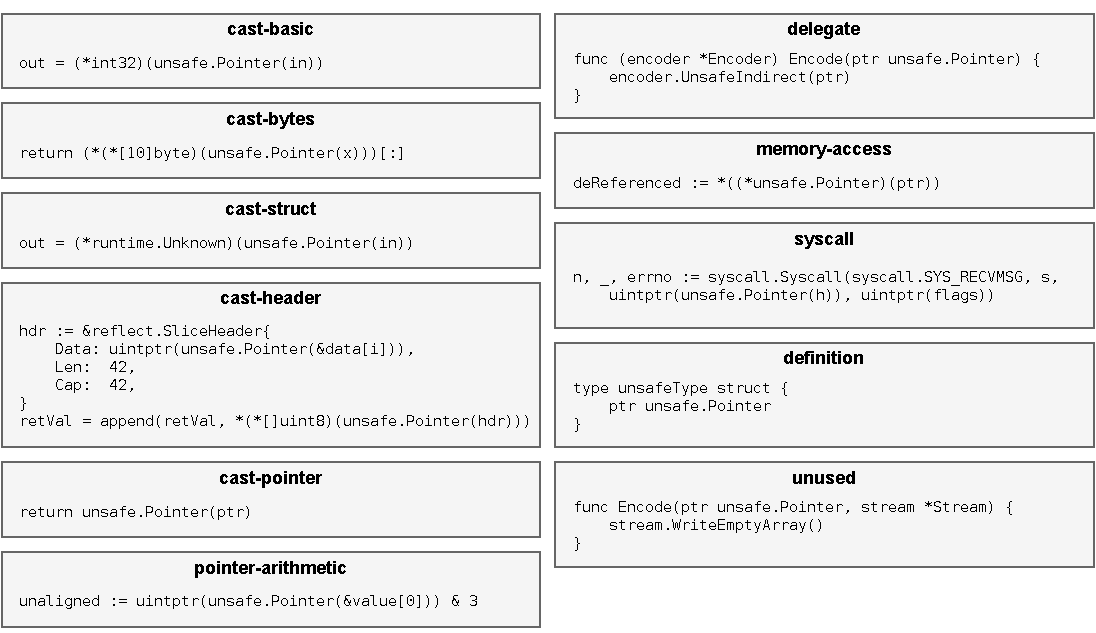
\includegraphics[width=\textwidth]{assets/figures/chapter4/usage-labels.pdf}
    \caption{Labeled data set usage classes}
    \label{fig:usage-labels}
\end{figure}


\begin{figure}[ht!]
    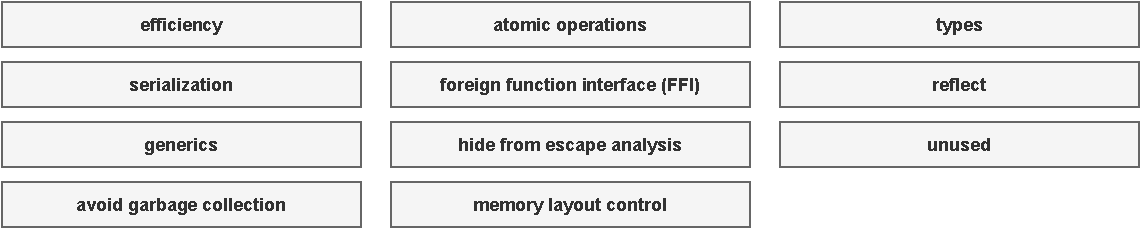
\includegraphics[width=\textwidth]{assets/figures/chapter4/purpose-labels.pdf}
    \caption{Labeled data set purpose classes}
    \label{fig:purpose-labels}
\end{figure}


Figure~\ref{fig:purpose-labels} shows the possible class labels in the purpose dimension.
The \textit{efficiency} class represents cases where \unsafe{} is used only to improve time or
space efficiency of the code.
Usages in this class could be rewritten to not use \unsafe{}.
The \textit{serialization} class includes (un)marshalling and (de)serialization operations like in-place casts between
complex types and bytes.
\textit{Generics} is applied where \unsafe{} is used to build functionality that would be implemented using generics if
they were available in current versions of Go.
Up until release \checkNum{1.15}, there is no support for generics in Go without additional libraries.
The \textit{avoid garbage collection} class contains usages to tell the Go compiler to lock a value while it is used,
for example, when calling a function written in assembly.
\textit{Atomic operations} is a class of usages of the atomic \acrshort{API}, which requires \unsafe{} for some of its
functions.
The \textit{foreign function interface} (\acrshort{FFI}) class includes all cases of interoperability with C code (CGo),
as well as calls to functions that receive their parameters as \unsafe{} pointers.
\textit{Hide from escape analysis} contains instances where \unsafe{} is used to deliberately exclude a value from being
seen by the \acrshort{EA} algorithm.
The \textit{memory layout control} class represents code used for low-level memory management.
\textit{Types} samples are used by the standard library for low-level implementation of the Go type system.
\textit{Reflect} includes instances of type reflection, as well as re-implementations of types contained in the regular
Go \textit{reflect} package, for example, to use \textit{unsafe.Pointer} instead of \textit{uintptr} for slice headers.
Lastly, \textit{unused} is a class for unused occurrences again.


%% ---------------------------------------------------------------------------------------------------------------------

\subsection{Purpose of \textit{Unsafe} in Practice (\ref{rq:purpose})}\label{subsec:go-geiger:qualitative-evaluation:purpose}

In this section, the novel labeled data set of \unsafe{} usages is used to answer~\ref{rq:purpose} about the purpose of
\unsafe{} in Go applications.
Table~\ref{tbl:dataset-classes} presents the number of samples for each class.
The columns denote the dimension of purpose, while the rows show the operation type dimension.
Columns are divided into separate counts for the \textit{app} and \textit{std} groups of samples.

\begin{table*}[htp!]
    \centering
    \caption[Labeled unsafe.Pointer usages in application code (non standard library) and standard library samples]
        {Labeled unsafe.Pointer usages in application code (non standard library) and standard library samples~\newline \tiny ~\newline \footnotesize
        \underline{eff}: efficiency, \underline{ser}: (de)serialization, \underline{gen}: generics,
        \underline{no GC}: avoid garbage collection, \underline{atomic}: atomic operations,
        \underline{FFI}: foreign function interface, \underline{HE}: hide from escape analysis, \underline{layout}: memory layout control,
        \underline{types}: Go type system,
        \underline{reflect}: type reflection, \underline{unused}: declared but unused \tiny ~\newline}
    \label{tbl:dataset-classes}
    \begin{adjustbox}{max width=\textwidth}
    
    %% do not paste from notebook, local changes done!
\begin{tabular}{r|cc|cc|cc|cc|cc|cc|cc|cc|cc|cc|cc|cc}
                    & \multicolumn{2}{c|}{\textbf{eff}} & \multicolumn{2}{c|}{\textbf{ser}} & \multicolumn{2}{c|}{\textbf{gen}} & \multicolumn{2}{c|}{\textbf{no GC}} & \multicolumn{2}{c|}{\textbf{atomic}} & \multicolumn{2}{c|}{\textbf{FFI}} & \multicolumn{2}{c|}{\textbf{HE}} & \multicolumn{2}{c|}{\textbf{layout}} & \multicolumn{2}{c|}{\textbf{types}} & \multicolumn{2}{c|}{\textbf{reflect}} & \multicolumn{2}{c|}{\textbf{unused}} & \multicolumn{2}{c}{\textbf{Total}} \\ %\hline
                    &  \textbf{app} &  \textbf{std} &  \textbf{app} &  \textbf{std} &  \textbf{app} &  \textbf{std} &   \textbf{app} &  \textbf{std} &    \textbf{app} &  \textbf{std} &  \textbf{app} &  \textbf{std} &  \textbf{app} &  \textbf{std} &    \textbf{app} &  \textbf{std} &   \textbf{app} &  \textbf{std} &     \textbf{app} &  \textbf{std} &    \textbf{app} &  \textbf{std} &   \textbf{app} &  \textbf{std} \\ \hline
                    
                   % \textbf{cast} & 562 & 16 & 178 & 33 & 18 & & & & & & 24 & 6 && 2 & 3 & 13 & & 45 & 1 & & & & 786 & 115 \\
        \textbf{cast-struct} &  401 &    4 &   50 &    6 &    6 &      &       &      &        &      &    6 &    2 &      &    2 &        &    4 &       &   31 &         &      &        &      &   463 &   49 \\
\rowcolor{verylightgray}
         \textbf{cast-basic} &   90 &    2 &   29 &    3 &    1 &      &       &      &        &      &    1 &    3 &      &      &      2 &    7 &       &    1 &         &      &        &      &   123 &   16 \\
                    \textbf{cast-header} &   36 &    1 &    3 &      &    1 &      &       &      &        &      &      &      &      &      &        &      &       &    3 &         &      &        &      &    40 &    4 \\
\rowcolor{verylightgray}
                    \textbf{cast-bytes} &   22 &    1 &   81 &   11 &      &      &       &      &        &      &    1 &      &      &      &      1 &      &       &    1 &         &      &        &      &   105 &   13 \\
                    \textbf{cast-pointer} &   13 &    8 &   15 &   13 &   10 &      &       &      &        &      &   16 &    1 &      &      &        &    2 &       &    9 &       1 &      &        &      &    55 &   33 \\
\rowcolor{verylightgray}
      \textbf{memory-access} &    2 &    1 &    9 &      &      &      &       &      &        &      &      &    1 &      &      &      4 &    6 &       &    4 &         &      &        &      &    15 &   12 \\
 \textbf{pointer-arithmetic} &    7 &    2 &    6 &    1 &      &      &       &      &        &    1 &      &    3 &    1 &    2 &      3 &    8 &       &    9 &         &      &        &      &    17 &   26 \\
\rowcolor{verylightgray}
         \textbf{definition} &    4 &    1 &   23 &      &    2 &      &       &      &        &      &    4 &    5 &      &      &        &    9 &       &    8 &       6 &    3 &        &      &    39 &   26 \\
           \textbf{delegate} &    4 &      &   64 &      &    2 &      &       &      &     11 &    5 &   29 &   45 &      &    4 &        &   14 &       &    6 &         &    1 &        &      &   110 &   75 \\
\rowcolor{verylightgray}
            \textbf{syscall} &      &      &      &      &      &      &    17 &  138 &        &      &      &      &      &      &        &      &       &      &         &      &        &      &    17 &  138 \\
             \textbf{unused} &      &      &      &      &      &      &       &      &        &      &      &      &      &      &        &      &       &      &         &      &     16 &    8 &    16 &    8 \\ \hline
%\rowcolor{verylightgray}
                  \textbf{total} &  579 &   20 &  280 &   34 &   22 &    0 &    17 &  138 &     11 &    6 &   57 &   60 &    1 &    8 &     10 &   50 &     0 &   72 &       7 &    4 &     16 &    8 &  1000 &  400 \\
\end{tabular}

    \end{adjustbox}
        \vspace{-10pt}
\end{table*}

The data shows that efficiency is by far the most prevalent reason to use \unsafe{} in real-world Go application code.
While these usages make up about \checkNum{58\%} of the application code samples, they account for only about
\checkNum{5\%} of the standard library usages.
Within the \textit{efficiency} class, casting operations cover most of the usages with \checkNum{97\%} (\textit{app})
and \checkNum{80\%} (\textit{std}) of the samples.
Next, the second most important motivation for \unsafe{} code in the application class is performing serialization or
deserialization operations, including marshalling of structured data to interchangeable formats.
This accounts for \checkNum{28\%} of the \textit{app} usages.
The standard library shows a different most common usage, which is avoiding garbage collection with \checkNum{35\%}.
This purpose is only found in \checkNum{2\%} of the \textit{app} samples.
Next, the \textit{type} (\checkNum{18\%}), \textit{\acrshort{FFI}} (\checkNum{15\%}), and \textit{memory layout}
(\checkNum{13\%}) classes are common in the \textit{std} samples.
A common distribution is the \textit{hide from escape analysis} class, which is rare both in the \textit{app}
(\checkNum{0.1\%}) and \textit{std} (\checkNum{2\%}) groups.
The same is true for the \textit{reflection} class (\checkNum{1\%} in both sets).
There are also only few samples (\checkNum{2\%}) that are used to implement generics functionality.
Some of the findings in the \textit{serialization} class could however be achieved with generics as well, so the classes
overlap slightly.

In conclusion, it is evident that the most important reasons to use \unsafe{} in Go applications are increasing
efficiency through in-place conversions, and serialization with direct casts.
Interestingly, both of them are achievable without \unsafe{} as well, so the code could be rewritten to remove these
usages.

\begin{answerToRQ}[\ref{rq:purpose}]
    \checkNum{More than half} of the \unsafe{} usages in projects and 3rd party libraries are to improve efficiency via
    \unsafe{} casts.
    In the Go standard library, \checkNum{every third} use of \unsafe{} is to avoid garbage collection.
\end{answerToRQ}


%% ---------------------------------------------------------------------------------------------------------------------

\section{Summary}\label{sec:go-geiger:summary}

With the \toolGeiger{} static analysis tool, this thesis contributes a tool to find and count \unsafe{} usages in Go
packages, including their dependencies.
Its design allows to distinguish usages by the context they appear in, which enables filtering and, thus, a focused
review of specific types such as function paramater declarations.
A study on \unsafe{} usage in \projsAnalyzed{} popular Go projects on \github{} revealed that while only about
\checkNum{a third} directly contain \unsafe{}, almost all of them import \unsafe{} code through their dependencies.

To study what operations are carried out using \unsafe{}, and for what purpose, a novel data set of
\numberLabeledCodeSnippets{} labeled code samples was presented.
It showed that the most common use cases are increasing efficiency by avoiding memory reallocations when converting
values between different types, serialization and marshalling, and control over the Go memory management system when
interacting with the foreign function interface (\acrshort{FFI}).
